\section{INTERCEPT TIMELINES}

\subsection{TERMINOLOGY}

\begin{tcoloritemize}
    \blueitem[Contact]
    \blueitem[Group]
    \blueitem[Picture]
\end{tcoloritemize}

\subsection[AR FLOW]{ACTIVE-RADAR MISSILE FLOW}

\begin{tcoloritemize}
    \blueitem[Launch-and-Leave]
    \blueitem[Launch-and-Decide]
\end{tcoloritemize}


\subsection{RANGE DEFINITIONS}

\begin{tcoloritemize}
    \blueitem[WEZ]
    \blueitem[MAR] \textbf{M}inimum \textbf{A}bort \textbf{R}ange

    \medskip
    minimum range at which fighter can perform an abort maneuver to kinematically defeat any launched bandit weapons 

    \blueitem[MSR] \textbf{M}inimum \textbf{S}hot \textbf{R}ange

    \medskip
    minimum range at which AIM-120 will go active before fighter reaches MAR if launched

    \blueitem[DOR] \textbf{D}esired \textbf{O}ut \textbf{R}ange
    \blueitem[TR] \textbf{T}ransition \textbf{R}ange
    \blueitem[MTR] \textbf{M}inimum \textbf{T}argeting \textbf{R}ange
    \blueitem[MRR] \textbf{M}inimum \textbf{R}ecommit \textbf{R}ange
    \blueitem[DR] \textbf{D}ecision \textbf{R}ange
\end{tcoloritemize}

\marginfigeometry

\subsection{SKATE TIMELINE}
\subsection{SHORT SKATE TIMELINE}
\subsection{BANZAI TIMELINE}

\marginpar{
    \captionsetup{type=figure}
    \centering
    \begin{tikzpicture}[figstyle]
        
        \draw[->] 
            (0,0) -- 
            node[below, pos=0]{
                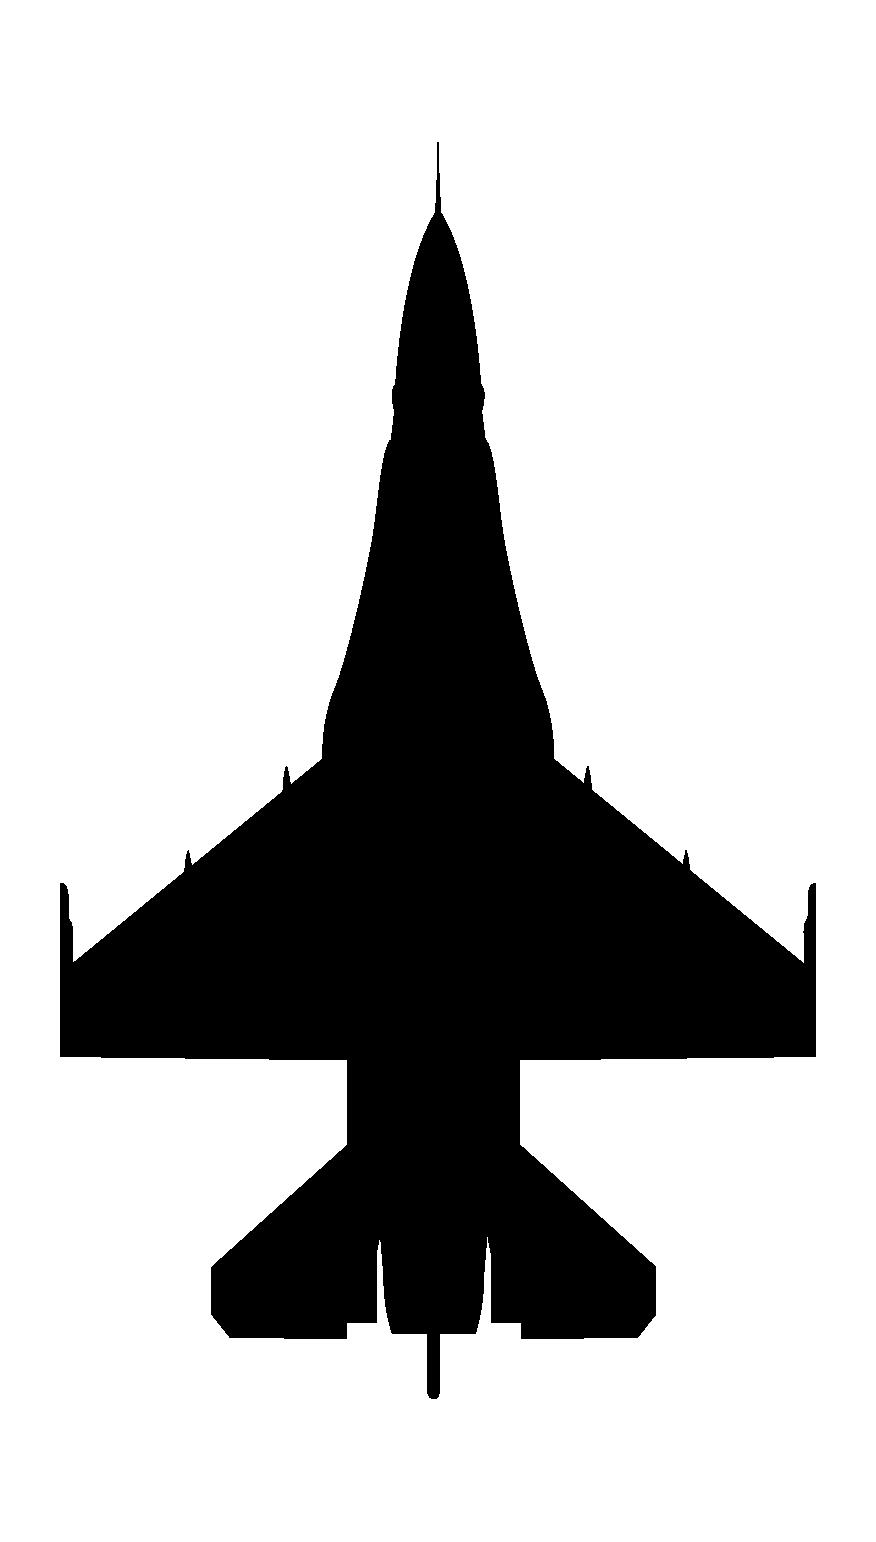
\includegraphics[
                width=7.5mm,
            ]{diagrams/aircraft/silhouette_f16_top.pdf}} 
            ++(0,20) 
            arc (180:90:5) 
            arc (-90:0:5) 
            -- ++(0,20) 
            arc (180:0:5) 
            -- ++(0,-50)
            node[below, pos=1, ]{
                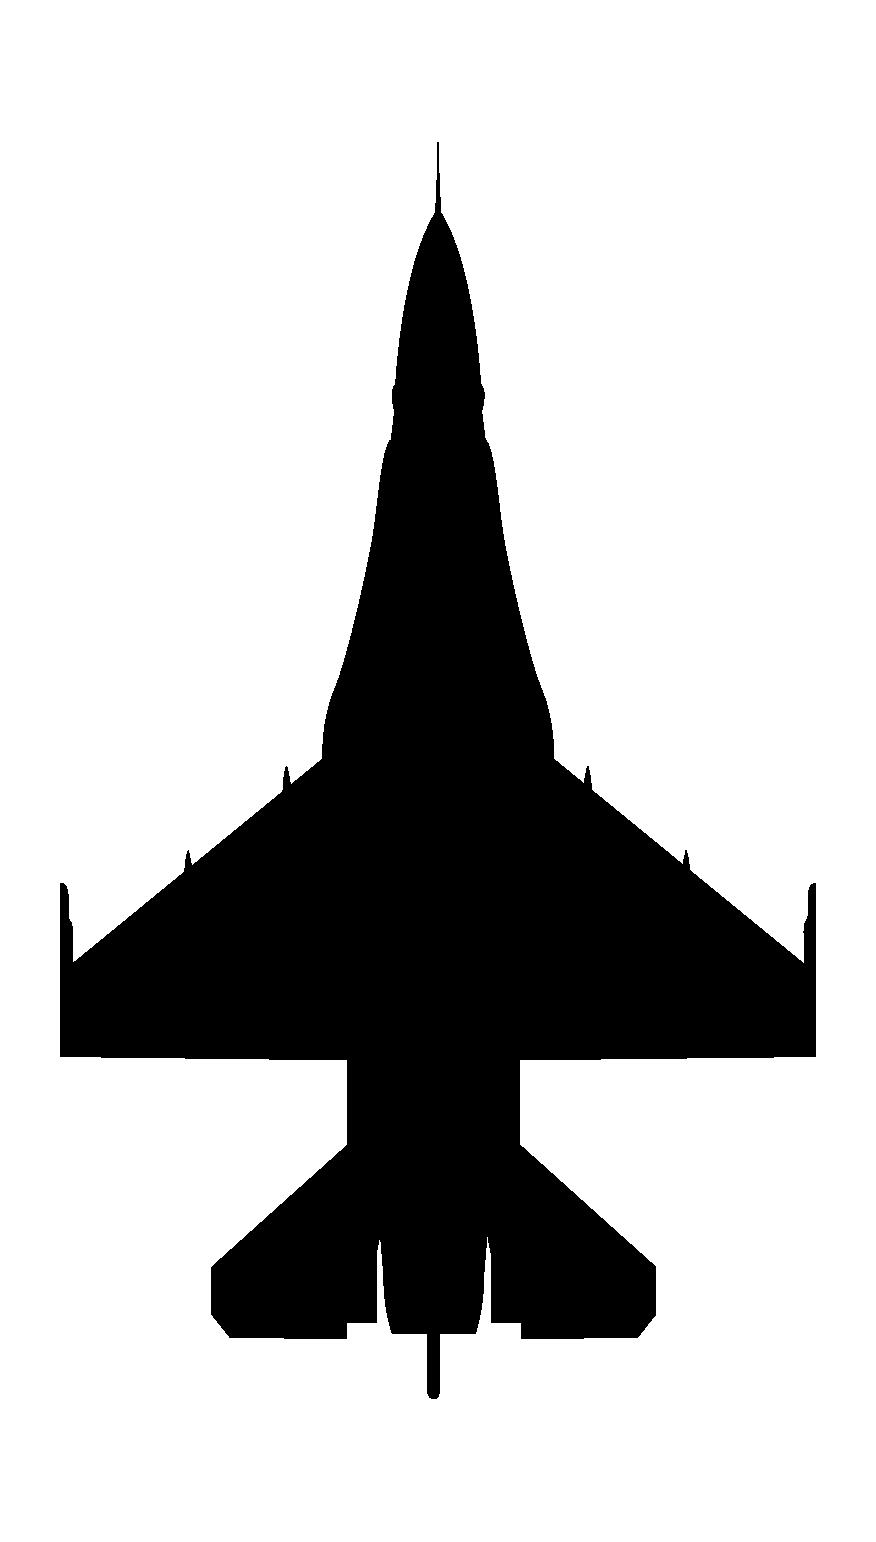
\includegraphics[
                    angle=180,
                    width=7.5mm,
            ]{diagrams/aircraft/silhouette_f16_top.pdf}};

    \end{tikzpicture}
    \caption{Work in progress timeline illustration}
}
\begin{center}
    \vspace{\textheight/4}
    \Large\titlefont\textbf{COMING SOON}
\end{center}

\marginfigrestore